\subsubsection{Electric Technic Motor 9v (ID: 2838)}
\begin{figure}[H]
  \centering
  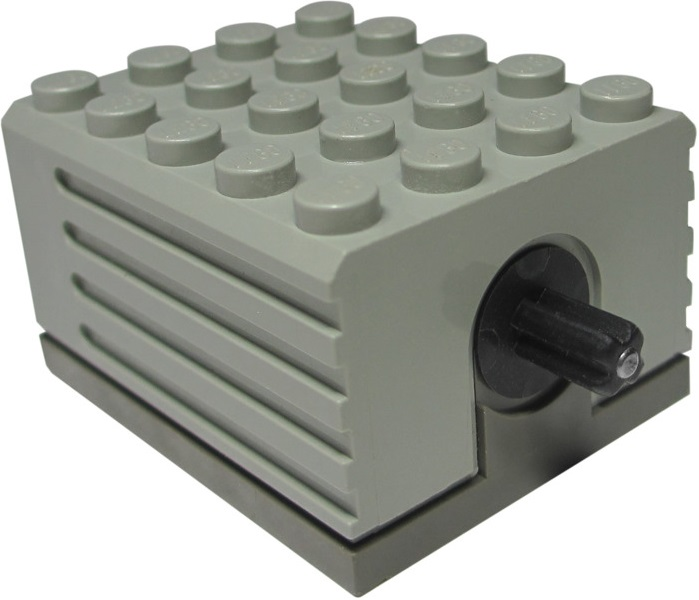
\includegraphics[width=3cm]{images/techAnalysis/LegoTechnicMotor.jpg}
  \caption{LEGO Technic Motor 9v \cite{BrickOWl-figure-Technic-Motor9v}}\label{fig:sssec:TechnicMotor}
\end{figure}
According to Philippe Hurbain, this motor, which can be seen in \autoref{fig:sssec:TechnicMotor}, is with its 4100rpm, a faster edition in the LEGO Technic universe, than the previously described Mini-motor.
However it is trading its speed with power, and is the weakest LEGO motor available.
Like the Mini-motor, this one does not have a built-in sensor, meaning that it does not allow for precise control in terms of degrees.
This motor also works by default on the EV3 and NXT 2.0 brick, through the RJ12 adapter cable, which is attached to the bottom middle of the motor. \cite{hurbain_lego_technicmotorComp}
